\chapter{Stable Neo-Hookean Flesh Simulation} \label{c:Paper}
In this chapter, I will examine further the topic of the paper \textit{\acrshort{snh}}. In the interest of understanding the thought process of the authors, I will include some of their calculations more detailed. In addition, examples and visualisations are presented for a better understanding. 

\section{Deformation Gradient}
In the following calculations the properties of the deformation gradient $\mathbf{F}$ covered in chapter 2 will be used. These properties are summarized in table \ref{table:gradient_quantities} for a better overview.

\begin{table}[!htbp]
\centering
    \begin{tabular}{ | l | l |}
    \hline
    \textbf{Symbol} & \textbf{Definition} \\ \hline
    $\mathbf{F} = \mathbf{RS}$ & Polar decomposition \\ \hline
    $J=\operatorname{det}(\mathbf{F})$ & Relative volume change \\ \hline
    $\mathbf{C}=\mathbf{F}^\intercal \mathbf{F}$ & Right Cauchy-Green  \\ \hline	
    $I_{C}=\operatorname{tr}(\mathbf{C})$ & First right Cauchy-Green invariant \\ \hline
    \end{tabular}
    \caption[Quantities derived from the Deformation Gradient]{Quantities derived from the Deformation Gradient \textbf{F}}
\label{table:gradient_quantities}
\end{table}


\section{Energy Formulation}
\subsection{Stability}
The core goal of the paper was to model deformations for virtual characters that have human-like features. In order to achieve better results than what has been done in current research, they formulated a new deformation energy. In chapter 2 I concluded that the appropriate energy for animating soft tissues as flesh has to be hyperelastic. An important property is the stability of the energy. We need an energy that is stable in the following four ways:

\textbf{1. Inversion Stability:} Given some arbitrary object, it is possible that while deforming the object we can arrive at a zero volume state or even an entire inversion. Take for example the tetrahedron shown in Fig. \ref{fig:inversion_1}. In Fig. \ref{fig:inversion_2} we see a deformed state of this tetrahedron where the volume is scaled down to zero and we are left with a simple triangle. In Fig. \ref{fig:inversion_3} we have an inversion of the object. The deformation energy has to be able to deal with both cases. That means that the energy has to be singularity-free and does not need any filters or threshold (\cite{Smith:2018:SNF:3191713.3180491}, 12:3).

\todoredefined[inline]{
TODO: Explain what last sentence means.
}

\begin{figure}[!ht]
\centering
\begin{subfigure}{.3\textwidth}
  \centering
  % include first image
  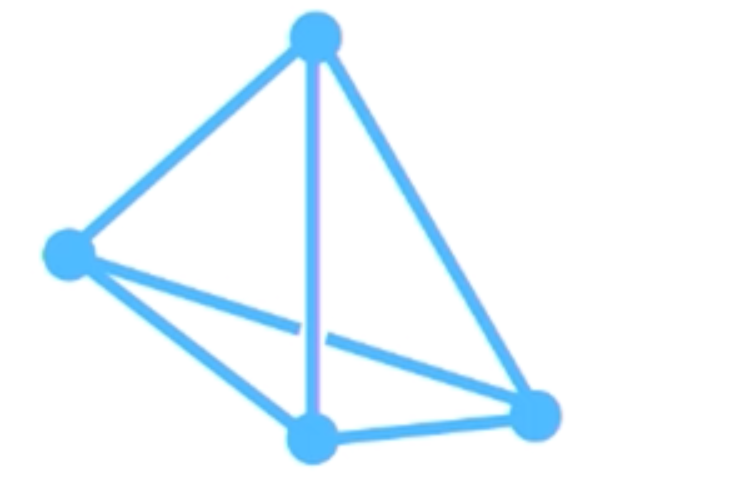
\includegraphics[width=.8\linewidth]{resources/inversion_1}  
  \caption{Rest state}
  \label{fig:inversion_1}
\end{subfigure}
\begin{subfigure}{.3\textwidth}
  \centering
  % include first image
  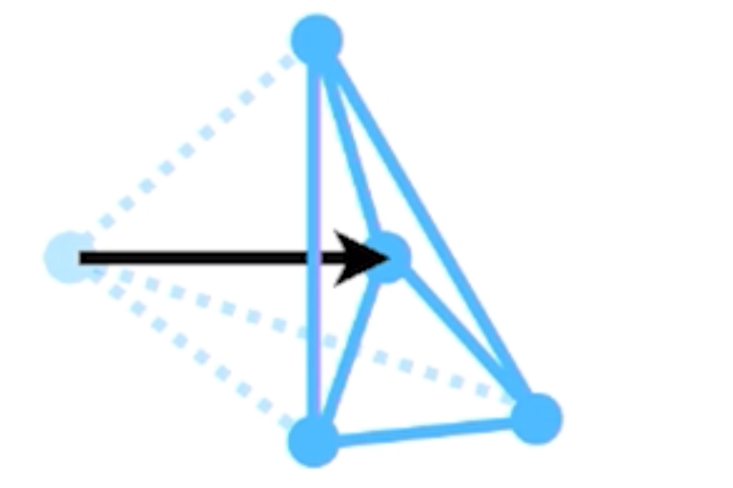
\includegraphics[width=.8\linewidth]{resources/inversion_2}  
  \caption{Zero-volume state}
  \label{fig:inversion_2}
\end{subfigure}
\begin{subfigure}{.3\textwidth}
  \centering
  % include second image
  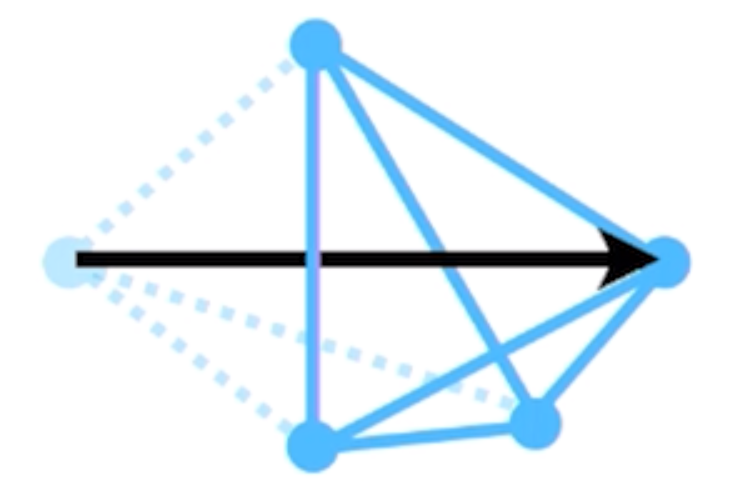
\includegraphics[width=.8\linewidth]{resources/inversion_3}  
  \caption{Inversed state}
  \label{fig:inversion_3}
\end{subfigure}
\caption[Inversion of a tetrahedron]{Inversion of a tetrahedron {\cite{STREAM2018}}}
\label{fig:inversion}
\end{figure}


\textbf{2. Reflection stability:} A reflection is a rotation around the coordinate origin. The deformation energy needs to be well behaved regardless of the reflection convention used in the singular value decomposition.
\todoredefined[inline]{
TODO: Explain a bit better what this means. What means well behaved?
}

\textbf{3. Rest stability:} When deforming an object in a certain way, we apply one or multiple forces to that object. When we achieve rest stability, we ensure that if the sum of all forces is equal to zero, the object must be back in its rest state.

\textbf{4. Meta-stability under degeneracy:} We can crush an object into an arbitrary shape like a plane, line or point. This process is illustrated for a cube in Fig. \ref{fig:meta_stability}. The cube should be able to recover to its actual shape after the deformation.

\begin{figure}[!htbp]
	\centering
	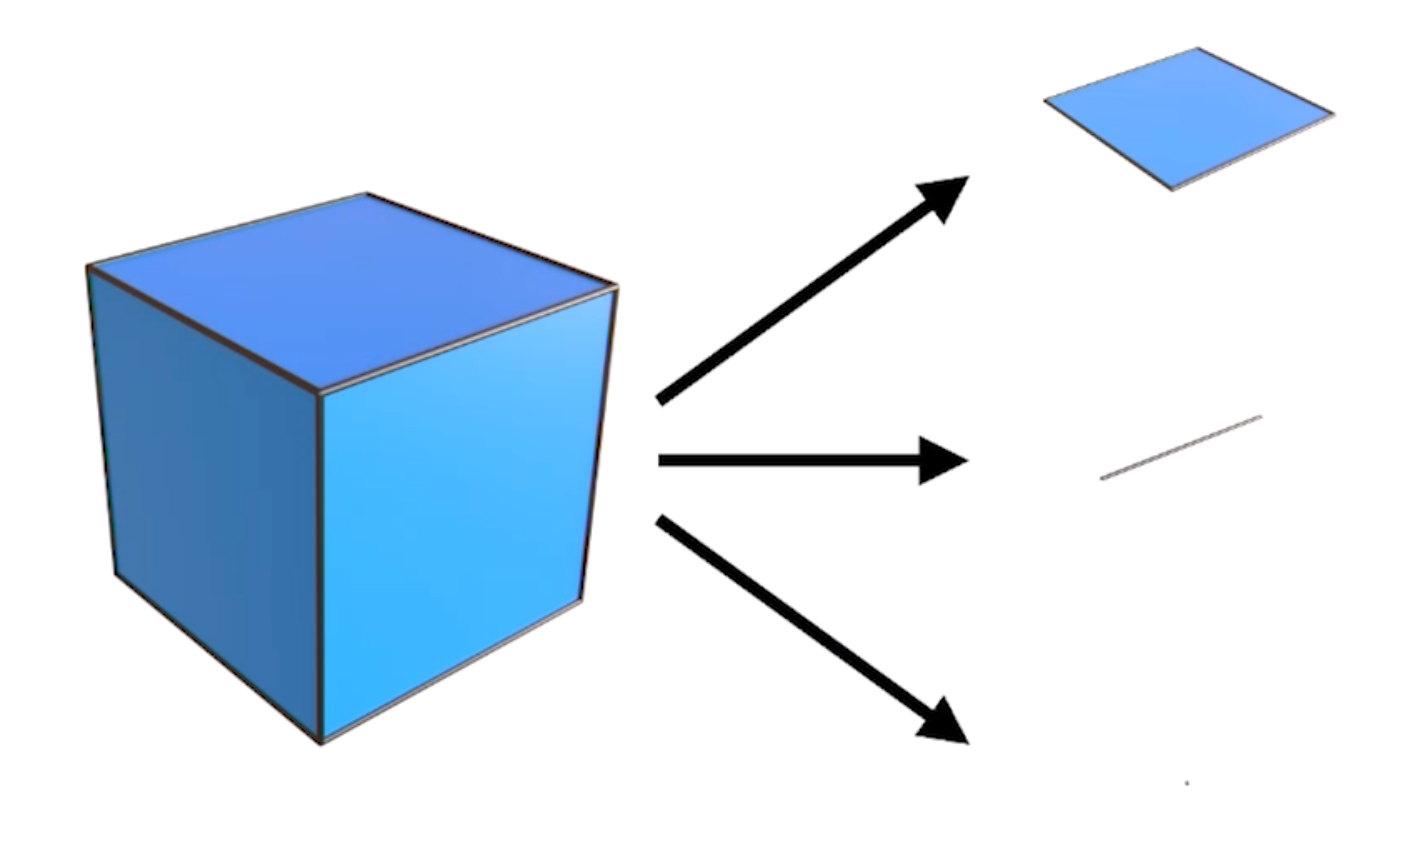
\includegraphics[width=0.5\textwidth]{resources/meta_stability}
	\caption[Illustration of meta stability]{Illustration of meta stability {\cite{STREAM2018}}}
	\label{fig:meta_stability}
\end{figure}

Based on these four requirements, we will in the following determine if a deformation energy is suited for our needs.

\todoredefined[inline]{
TODO: Maybe add own images and more sources.
}

\subsection{Existing Neo-Hookean Energies}

In previous literature, a few energies were proposed that I will analyse in this section. They are listed in table \ref{table:energies} below.

\begin{table}[!htbp]
\centering
    \begin{tabular}{ | l | l |}
    \hline
    \textbf{Energy} & \textbf{Author(s)} \\ \hline
    $\Psi_{Neo}=\frac{\mu}{2}\left(I_{C}-3\right)-\mu \log J+\frac{\lambda}{2}(\log J)^{2}$ & e.g. Bonet and Wood 2008 \\ \hline
    $\Psi_{\mathrm{A}}=\frac{\mu}{2}\left(I_{C}-3\right)-\mu \log J+\frac{\lambda}{2}(J-1)^{2}$ & Odgen 1997 \\ \hline
    $\Psi_{\mathrm{B}}=\frac{\mu}{2}\left(J^{-2 / 3} I_{C}-3\right)+\frac{\lambda}{2}(J-1)^{2}$ & Bower 2009 \\ \hline
    $\Psi_{\mathrm{C}}=\frac{\mu}{2}\left(J^{-2 / 3} I_{C}-3\right)+\frac{\lambda}{2}(J-1)^{2}$ & Wang and Yang 2016 \\ \hline
    \end{tabular}
    \caption[Summary of proposed energies]{Summary of proposed energies (\cite{Smith:2018:SNF:3191713.3180491}, 12:3)}
\label{table:energies}
\end{table}

Each energy formulation can be split up into a 1D length term and a 3D volume term. The 1D length term penalizes the length changes an object undergoes, whereas the 3D volume term is a volume-preserving penalty term.

\begin{table}[!htbp]
\centering
    \begin{tabular}{ | l | l | l |}
    \hline
    \textbf{Energy} & \textbf{1D length term} & \textbf{3D volume term} \\ \hline
    $\Psi_{Neo}$ & $\frac{\mu}{2}\left(I_{C}-3\right)$ & $-\mu \log J+\frac{\lambda}{2}(\log J)^{2}$ \\ \hline
    $\Psi_{\mathrm{A}}$ & $\frac{\mu}{2}\left(I_{C}-3\right)$ & $-\mu \log J+\frac{\lambda}{2}(J-1)^{2}$ \\ \hline
    $\Psi_{\mathrm{B}}$ & $\frac{\mu}{2}\left(J^{-2 / 3} I_{C}-3\right)$ & $\frac{\lambda}{2}(J-1)^{2}$ \\ \hline
    $\Psi_{\mathrm{C}}$ & $\frac{\mu}{2}\left(J^{-2 / 3} I_{C}-3\right)$ & $\frac{\lambda}{2}(J-1)^{2}$ \\ \hline
    \end{tabular}
    \caption{Energies split up into their 1D length and 3D volume term}
\label{table:energies_split}
\end{table}

\subsubsection{1D Length Term}
Mooney (\cite{mooney1940theory}) originally proposed the 1D length term 
\[
\Psi_{M}=\frac{\mu}{2}\left(I_{C}-3\right)
\]
that is used in $\Psi_{Neo}$ and $\Psi_{A}$. If we expand the energy with the singular values of the deformation gradient \textbf{F}, we get the following term:
\[
\Psi_{M}=\frac{\mu}{2}\left(\sigma_{0}^2 + \sigma_{1}^2 + \sigma_{2}^2 - 3\right)
\]
This energy reaches its minimum at a zero volume state, meaning $I_{C}=0$ which results in $\Psi_{M}=-3$. Mooney added the hard constraint that $J=1$, so that the energy is minimized at the volume preserving configuration that is closest to the stretch space origin. Note that the energy is singularity free and well defined under inversion.

The second term 
\[
\Psi_{R} = \frac{\mu}{2}\left(J^{-2 / 3} I_{C}-3\right)
\]
is used in $\Psi_{B}$ and $\Psi_{C}$ and was introduced by Rivlin (\cite{rivlin1948large}). Using the singular values of \textbf{F}, we get the following term:
\[
\Psi_{R} = \frac{\mu}{2}\left(\frac{\sigma_{0}^2 + \sigma_{1}^2 + \sigma_{2}^2}{(\sigma_{0}  \sigma_{1}  \sigma_{2})^\frac{2}{3}}
 - 3\right)
\]
Unfortunately this term is not singularity free. If either $\sigma_{0}$, $\sigma_{1}$ or $\sigma_{2}$ is equal to zero the result is not defined anymore.

\subsubsection{3D Volume Term}
The volume term of $\Psi_{Neo}$, meaning
\[
\Psi_{Neo, volume} = -\mu \log J+\frac{\lambda}{2}(\log J)^{2}
\]
results in some numerical problems since the logarithmic function is not defined for $J<0$ and grows unbounded for $J \rightarrow 0$. In conclusion $\Psi_{Neo, volume}$ is not singularity free. 
The same applies for the 3D volume term of $\Psi_{A}$, namely
\[
\Psi_{A, volume} = -\mu \log J+\frac{\lambda}{2}(J-1)^{2}.
\]
The term of $\Psi_{A}$ and $\Psi_{B}$ which is of the form
\[
\Psi_{M} = \frac{\lambda}{2}(J-1)^{2}
\]
does not have these problems. It is bounded, well defined and invertible. After these observations we combine the robust length with the robust volume term and receive $\Psi_D$ that is defined as
\[
\Psi_{D} = \frac{\mu}{2}\left(I_{C}-3\right) +\frac{\lambda}{2}(J-1)^{2}
\]
and is singularity free and well defined under inversion. Unfortunately, $\Psi_D$ does not satisfy the requirement of being rest stable which will be discussed in the next section.

\todoredefined[inline]{
TODO: Bonet and Wood 2008 or 1997?
}

\subsection{Rest Stabilization}
Although $\Psi_{D}$ meets almost all stated requirements, it is not rest stable. This can be shown with the Piola-Kirchhoff (PK1) stress tensor for $\Psi_D$ derived by the deformation gradient \textbf{F}:
\begin{align*}
P_{D}(\mathbf{I}) &= \frac{\partial \Psi_{D}}{\partial \mathbf{F}} (\mathbf{I}) = \frac{\partial \Psi_{D}}{\partial \mathbf{F}} \left[ \frac{\mu}{2}\left(I_{C}-3\right) +\frac{\lambda}{2}(J-1)^{2} \right] \\
&= \frac{\partial \Psi_{D}}{\partial \mathbf{F}}  \frac{\mu}{2}\left(\operatorname{tr}(\mathbf{I}^\intercal \mathbf{I})-3\right) +\frac{\partial \Psi_{D}}{\partial \mathbf{F}} \frac{\lambda}{2}(\operatorname{tr}(\mathbf{I})-1)^{2} \\
&= \mu I + \lambda (\operatorname{det}(\mathbf{I})-1)  \frac{\partial}{\partial \mathbf{F}} \operatorname{det}(\mathbf{I}) = \mu \mathbf{I} \neq 0
\end{align*}

If the energy had rest stability, $P_{D}(\mathbf{I})$ would resolve to zero. Unfortunately, this is not the case here. In order to solve that problem, the authors modified $(J-1)^{2}$ to $(J-\alpha)^{2}$. Using this modification the energy can written as
\[
\Psi_{E} = \frac{\mu}{2}\left(I_{C}-3\right) +\frac{\lambda}{2}(J-\alpha)^{2}.
\]

Inserting $\Psi_E$ into the PK1 equation from before, we get
\begin{align*}
P_{E}(\mathbf{F}) &= \frac{\partial \Psi_{E}}{\partial \mathbf{F}} \left[ \frac{\mu}{2}\left(I_{C}-3\right) +\frac{\lambda}{2}(J-\alpha)^{2} \right] \\
&= \mu \mathbf{F} + \lambda (\operatorname{det}(\mathbf{F})-\alpha)  \frac{\partial}{\partial \mathbf{F}} \operatorname{det}(\mathbf{F}).
\end{align*}
Solving for an alpha that satisfies $P_{E}(\mathbf{I})=0$ gives us $\alpha=1+\frac{\mu}{\lambda}$. Now $\Psi_{E}$ has to be changed accordingly:
\begin{align*}
\Psi_{E} &= \frac{\mu}{2}\left(I_{C}-3\right) +\frac{\lambda}{2}(J-1-\frac{\mu}{\lambda})^{2} \\
&= \frac{\mu}{2}\left(I_{C}-3\right) - \mu\left(J-1\right) + \frac{\lambda}{2}(J-1)^{2} + \left(\frac{\mu}{\lambda}\right)^{2}.
\end{align*}
Since constants disappear under differentiation this expression is functionally equivalent to 
\[
\Psi_{E} = \frac{\mu}{2}\left(I_{C}-3\right) - \mu\left(J-1\right) + \frac{\lambda}{2}(J-1)^{2}.
\]
Now we can see that $\Psi_{E}$ looks very similar to $\Psi_{Neo}$. The difference is that $log(J)$ is replaced with $(J-1)$ in $\Psi_{E}$. Keep in mind that $(J-1)$ is the first term in the taylor approximation of $\operatorname{log}(J)$ at $J=1$:
\begin{align*}
\sum_{n=0}^{\infty} &= \frac{f^{(n)}(1)}{n!} (J-1)^{n} \\
&= \boldsymbol{(J-1)} - \frac{1}{2} (J-1)^{2} + \frac{1}{3} (J-1)^{3} -\frac{1}{4} (J-1)^{4} + \text{...}
\end{align*}
Thus $\Psi_{E}$ is an approximation of $\Psi_{Neo}$.

\todoredefined[inline]{
TODO: Add "Zwischenschritte"? Include all calculations? Do we need a bit of a better conclusion of what we did (taylor, neo, sing. free, rest stable)? Check consistency of calculations (when trace when $I_C$ etc.).
}

\subsection{Meta-Stability under Degeneracy}
The final energy is
\begin{equation}\label{eq:stable_energy}
\Psi_{new} = \frac{\mu}{2}\left(I_{C}-3\right) + \frac{\lambda}{2}(J-\alpha)^{2} - \frac{\mu}{2} \operatorname{log}\left(I_{C}+1\right).
\end{equation}
With that adjustment the rest stability term can be written as $\alpha=1+\frac{\mu}{\lambda}-\left(\frac{\mu}{4}\right)\lambda$.

\todoredefined[inline]{
TODO: How much needs to be explained here?
}

\subsection{Lamé Reparametrization}
\todoredefined[inline]{
TODO: How much needs to be explained here?
}


\section{Energy Analysis}
The goal of this chapter is to show that a complete eigenanalysis can be performed on Eq. \ref{eq:stable_energy}.


\subsection{First Piola-Kirchhoff Stress (PK1)}
In order to analyse the energy PK1 can be used for Eq. \ref{eq:stable_energy}:
\begin{align*}
P(\mathbf{F}) &= \frac{\partial \Psi_{D}}{\partial \mathbf{F}} \left[ \frac{\mu}{2}\left(I_{C}-3\right) + \frac{\lambda}{2}(J-\alpha)^{2} - \frac{\mu}{2}\left(I_{C}+1\right) \right] \\
&= \mu \mathbf{F} + \lambda (\operatorname{det}(\mathbf{F})-\alpha)  \frac{\partial}{\partial \mathbf{F}} \operatorname{det}(\mathbf{F}) - \frac{\partial}{\partial \mathbf{F}} \left[\operatorname{log}\left(\operatorname{tr}(\mathbf{F}^\intercal \mathbf{F})+1\right)\right] \\
&= \mu \mathbf{F} + \lambda (\operatorname{det}(\mathbf{F})-\alpha)  \frac{\partial}{\partial \mathbf{F}} \operatorname{det}(\mathbf{F}) - \mu \mathbf{F} \frac{1}{\operatorname{tr}(\mathbf{F}^\intercal \mathbf{F}) + 1} \\
&= \mu \left( 1 - \frac{1}{\operatorname{tr}(\mathbf{F}^\intercal \mathbf{F}) + 1}\right) \mathbf{F} + \lambda(J-\alpha)\frac{\partial J}{\partial \mathbf{F}}
\end{align*}

with $\alpha=1+\frac{\mu}{\lambda}-\left(\frac{\mu}{4}\right)\lambda$. For further use it can be more practical to write $\frac{\partial J}{\partial \mathbf{F}}$ as a result of cross products:
\begin{equation}\label{eq:cross_product}
\frac{\partial J}{\partial \mathbf{F}} = \left[ \,f_1 \times f_2\, \bigg| \,f_2 \times f_0\, \bigg| \,f_0 \times f_1\, \right].
\end{equation}

\todoredefined[inline]{
TODO: Is it easy to follow? Maybe add some explanations of some steps? Maybe move cross product into background instead of here.
}

\subsection{The Energy Hessian Terms}
Using the scalar notation for $\mathbf{F}$, the Hessian of the energy can be written as a fourth-order matrix-of-matrices:
\[
\frac{\partial^2 \psi}{\partial \mathbf{F}^2} = \frac{\partial P(\mathbf{F})}{\partial \mathbf{F}} = 
\left[\begin{array}{ccc}{\left[\frac{\partial P(\mathbf{F})}{\partial f_0}\right]} & {\left[\frac{\partial P(\mathbf{F})}{\partial f_3}\right]} & {\left[\frac{\partial P(\mathbf{F})}{\partial f_6}\right]} \\ {\left[\frac{\partial P(\mathbf{F})}{\partial f_1}\right]} & {\left[\frac{\partial P(\mathbf{F})}{\partial f_4}\right]} & {\left[\frac{\partial P(\mathbf{F})}{\partial f_7}\right]} \\ {\left[\frac{\partial P(\mathbf{F})}{\partial f_2}\right]} & {\left[\frac{\partial P(\mathbf{F})}{\partial f_5}\right]} & {\left[\frac{\partial P(\mathbf{F})}{\partial f_8}\right]} \end{array}\right]
\]

in which each entry is defined as
\[
\frac{\partial P(\mathbf{F})}{\partial f_i} = \frac{\partial}{\partial f_i} \left[ \mu \left( 1 - \frac{1}{\operatorname{tr}(\mathbf{F}^\intercal \mathbf{F}) + 1}\right) \mathbf{F} + \lambda(J-\alpha)\frac{\partial J}{\partial \mathbf{F}} \right]
\]
\[
\stackrel{\text{prod.rule}}{=} \underbrace{\frac{\partial \mathbf{F}}{\partial f_i} \mu \left( 1 - \frac{1}{\operatorname{tr}(\mathbf{F}^\intercal \mathbf{F}) + 1}\right)}_{\mathrm{T}_{i}}  + \underbrace{\mathbf{F} \mu \frac{2}{\left(\operatorname{tr}(\mathbf{F^\intercal}\mathbf{F}) + 1\right)^2} f_i}_{_{\mathrm{M}_{i}}}
\]
\[
r+ \underbrace{\lambda \frac{\partial J}{\partial f_i} \frac{\partial J}{\partial \mathbf{F}}}_{_{\mathrm{G}_{i}}}+ \underbrace{\lambda (J- \alpha) \frac{\partial^2 J}{\partial \mathbf{F}\partial f_i}}_{_{\mathrm{H}_{i}}} \in \mathbb{R}^{3}.
\]
We can split up this final equation into these four term: $\mathrm{T}_i$ (Tikohonov), $\mathrm{M}_i$ (Mu), $\mathrm{G}_i$ (Volume Gradient), $\mathrm{H}_i$ (Volume Hessian). I will examine them separately in the next section.

\subsection{The Tikhonov, Mu, and Gradient Terms}
\subsubsection{Tikhonov}
The Tikhonov term is a fourth-order matrix-of-matrices
\[
\mathbb{T} = \frac{\partial \mathbf{F}}{\partial f_i} = \left[\begin{array}{ccc}{\begin{bmatrix} 1 & 0 & 0 \\ 0 & 0 & 0 \\ 0 & 0 & 0 \end{bmatrix}} & {\begin{bmatrix} 0 & 1 & 0 \\ 0 & 0 & 0 \\ 0 & 0 & 0 \end{bmatrix}} & {\begin{bmatrix} 0 & 0 & 1 \\ 0 & 0 & 0 \\ 0 & 0 & 0 \end{bmatrix}} \\ {\begin{bmatrix} 0 & 0 & 0 \\ 1 & 0 & 0 \\ 0 & 0 & 0 \end{bmatrix}} & {\begin{bmatrix} 0 & 0 & 0 \\ 0 & 1 & 0 \\ 0 & 0 & 0 \end{bmatrix}} & {\begin{bmatrix} 0 & 0 & 0 \\ 0 & 0 & 1 \\ 0 & 0 & 0 \end{bmatrix}} \\ {\begin{bmatrix} 0 & 0 & 0 \\ 0 & 0 & 0 \\ 1 & 0 & 0 \end{bmatrix}} & {\begin{bmatrix} 0 & 0 & 0 \\ 0 & 0 & 0 \\ 0 & 1 & 0 \end{bmatrix}} & {\begin{bmatrix} 0 & 0 & 0 \\ 0 & 0 & 0 \\ 0 & 0 & 1 \end{bmatrix}} \end{array}\right].
\]
If we vectorize $\mathbb{T}$, we get the identity matrix $\mathbf{I} \in \mathbb{R}^{9x9}$ which is of full rank, positive definite and independent of the values in \textbf{F}. 
\[
\operatorname{vec}(\mathbb{T}) =  \mathbf{\check{T}} = \mathbf{I} = \in \mathbb{R}^{9x9}.
\]
It serves as a regularizer for the rest of the energy.

\subsubsection{Mu}
The Mu term has the same structure with different entries
\[
\mathbb{M} = \mathbf{F} f_i = \left[\begin{array}{ccc}{\begin{bmatrix} f_0^2 & f_0f_3 & f_0f_6 \\ f_0f_1 & f_0f_4 & f_0f_7 \\ f_0f_2 & f_0f_5 & f_0f_8 \end{bmatrix}} & {\begin{bmatrix} f_3f_0 & f_3^2 & f_3f_6 \\ f_3f_1 & f_3f_4 & f_3f_7 \\ f_3f_2 & f_3f_5 & f_3f_8 \end{bmatrix}} & {\begin{bmatrix} f_6f_0 & f_6f_3 & f_6f_6 \\ f_6f_1 & f_6f_4 & f_6f_7 \\ f_6f_2 & f_6f_5 & f_6f_8 \end{bmatrix}} \\ {\begin{bmatrix} f_1f_0 & f_1f_3 & f_1f_6 \\ f_1^2 & f_1f_4 & f_1f_7 \\ f_1f_2 & f_1f_5 & f_1f_8 \end{bmatrix}} & {\begin{bmatrix} f_4f_0 & f_4f_3 & f_4f_6 \\ f_4f_1 & f_4^2 & f_4f_7 \\ f_4f_2 & f_4f_5 & f_4f_8 \end{bmatrix}} & {\begin{bmatrix} f_7f_0 & f_7f_3 & f_7f_6 \\ f_7f_1 & f_7f_4 & f_7^2 \\ f_7f_2 & f_7f_5 & f_7f_8 \end{bmatrix}} \\ {\begin{bmatrix} f_2f_0 & f_2f_3 & f_2f_6 \\ f_2f_1 & f_2f_4 & f_2f_7 \\ f_2^2 & f_2f_5 & f_2f_8 \end{bmatrix}} & {\begin{bmatrix} f_5f_0 & f_5f_3 & f_5f_6 \\ f_5f_1 & f_5f_4 & f_5f_7 \\ f_5f_2 & f_5^2 & f_5f_8 \end{bmatrix}} & {\begin{bmatrix} f_8f_0 & f_8f_3 & f_8f_6 \\ f_8f_1 & f_8f_4 & f_8f_7 \\ f_8f_2 & f_8f_5 & f_8^2 \end{bmatrix}} \end{array}\right].
\]
When vectorizing $\mathbb{M}$, the resulting matrix $\mathbf{\check{M}}$ has the squared values of $f_i$ placed on the diagonal
\[
\operatorname{vec}(\mathbb{M})= \mathbf{\check{M}} = \begin{bmatrix} f_0^2 & f_1f_0 & f_2f_0 & f_3f_0 & f_4f_0 & f_5f_0 & f_6f_0 & f_7f_0 & f_8f_0 \\ f_0f_1 & f_1^2 & f_2f_1 & f_3f_1 & f_4f_1 & f_5f_1 & f_6f_1 & f_7f_1 & f_8f_1 \\ f_0f_2 & f_1f_2 & f_2^2 & f_3f_2 & f_4f_2 & f_5f_2 & f_6f_2 & f_7f_2 & f_8f_2 \\ f_0f_3 & f_1f_3 & f_2f_3 & f_3^2 & f_4f_3 & f_5f_3 & f_6f_3 & f_7f_3 & f_8f_3 \\ f_0f_4 & f_1f_4 & f_2f_4 & f_3f_4 & f_4^2 & f_5f_4 & f_6f_4 & f_7f_4 & f_8f_4 \\ f_0f_5 & f_1f_5 & f_2f_5 & f_3f_5 & f_4f_5 & f_5^2 & f_6f_5 & f_7f_5 & f_8f_5 \\ f_0f_6 & f_1f_6 & f_2f_6 & f_3f_6 & f_4f_6 & f_5f_6 & f_6^2 & f_7f_6 & f_8f_6 \\ f_0f_7 & f_1f_7 & f_2f_7 & f_3f_7 & f_4f_7 & f_5f_7 & f_6f_7 & f_7^2 & f_8f_7 \\ f_0f_8 & f_1f_8 & f_2f_8 & f_3f_8 & f_4f_8 & f_5f_8 & f_6f_8 & f_7f_8 & f_8^2 \end{bmatrix}.
\]
This structure makes it possible to write $\mathbf{\check{M}}$ as an outer product of $\operatorname{vec}(\mathbf{F})$
\[
\mathbf{\check{M}}= \operatorname{vec}(\mathbf{F})\operatorname{vec}(\mathbf{F})^\intercal = \mathbf{\check{f}} \mathbf{\check{f}}^\intercal.
\]
This matrix has rank one and has a single non-zero eigenvalue. In order to examine the eigenvalues, we can calculate
\[
\| \mathbf{\check{f}} \|^{2}_{2} = \sum_{n=0}^8 | f_n |^2 = \| \mathbf{F} \|^{2}_{F} = \sum_{n=0}^3 \sigma^2_i = \left( \sigma_0^2 + \sigma_1^2 + \sigma_2^2 \right)
\]
in which $\|\cdot\|_F$ stands for the Frobenius norm introduced in Def. \ref{FN} and $\sigma_i$ for the singular values from $\mathbf{\Sigma}$ in the SVD of $\mathbf{F}$ stated in Eq. \ref{eq:svd_simga}. The equation can be obtained by using Eq. \ref{eq:FN}. The eigenvector is $\mathbf{\check{f}} / \| \mathbf{\check{f}} \|$. The eigenvalue is always non-negative and large if $\mathbf{F}$ contains a large strech.

\subsubsection{Gradient}
The gradient term also has the same structure as the two terms before with different entries defined by
\[
\mathbb{G}(\mathbf{F}) = \frac{\partial J}{\partial \mathbf{F}} \frac{\partial J}{\partial fi}.
\]
The vectorized matrix $\mathbf{\check{G}}$ can be written in a similar form as for the Mu term. With the help of the cross product of $\partial J / \partial \mathbf{F}$ stated in Eq. \ref{eq:cross_product}, $\mathbf{\check{G}}$ can be written as an outer product in the following way:
\[
\operatorname{vec}(\mathbb{G}(\mathbf{F})) = \mathbf{\check{G}} = \operatorname{vec}\left(\frac{\partial J}{\partial \mathbf{F}}\right) \operatorname{vec}\left(\frac{\partial J}{\partial \mathbf{F}}\right)^\intercal = \mathbf{\check{g}} \mathbf{\check{g}}^\intercal.
\]
As in the Mu term, we again have a single non-zero, non-negative eigenvalue calculated by
\[
\| \mathbf{\check{g}} \|^2_2 = \left\| \frac{\partial J}{\partial \mathbf{F}} \right \|^2_F = \left[ (\sigma_0 \sigma_1)^2 + (\sigma_0 \sigma_2)^2 + (\sigma_1 \sigma_2)^2 \right].
\]
The eigenvector is $\mathbf{\check{g}} / \| \mathbf{\check{g}} \|$.

\todoredefined[inline]{
TODO: Not all proofs and calculations included. Add or leave out some if too confusing.
}


\subsection{The Volume Hessian}
The volume Hessian term is of the form
\[
\mathbb{H} = \frac{\partial^2 J}{\partial \mathbf{F} \partial f_i} = \left[\begin{array}{ccc}{\frac{\partial}{\partial \mathbf{F}}\left[\frac{\partial J}{\partial f_0}\right]} & {\frac{\partial}{\partial \mathbf{F}}\left[\frac{\partial J}{\partial f_3}\right]} & {\frac{\partial}{\partial \mathbf{F}}\left[\frac{\partial J}{\partial f_6}\right]} \\ {\frac{\partial}{\partial \mathbf{F}}\left[\frac{\partial J}{\partial f_1}\right]} & {\frac{\partial}{\partial \mathbf{F}}\left[\frac{\partial J}{\partial f_4}\right]} & {\frac{\partial}{\partial \mathbf{F}}\left[\frac{\partial J}{\partial f_7}\right]} \\ {\frac{\partial}{\partial \mathbf{F}}\left[\frac{\partial J}{\partial f_2}\right]} & {\frac{\partial}{\partial \mathbf{F}}\left[\frac{\partial J}{\partial f_5}\right]} & {\frac{\partial}{\partial \mathbf{F}}\left[\frac{\partial J}{\partial f_8}\right]} \end{array}\right].
\]
Vectorizing $\mathbb{H}$ reveals the structure
\[
\operatorname{vec}(\mathbb{H}) = \mathbf{\check{H}} = \begin{bmatrix} 0 & 0 & 0 & 0 & f_8 & 0 & 0 & -f_5 & f_4 \\ 0 & 0 & 0 & -f_8 & 0 & f_6 & f_5 & 0 & -f_3 \\ 0 & 0 & 0 & f_7 & -f_6 & 0 & -f_4 & f_3 & 0 \\ 0 & -f_8 & f_7 & 0 & 0 & 0 & 0 & f_2 & -f_1 \\ f_8 & 0 & -f_6 & 0 & 0 & 0 & -f_2 & 0 & f_0 \\ -f_7 & f_6 & 0 & 0 & 0 & 0 & f_1 & -f_0 & 0 \\ 0 & f_5 & -f_4 & 0 & -f_2 & f_1 & 0 & 0 & 0 \\ -f_5 & 0 & f_3 & f_2 & 0 & -f_0 & 0 & 0 & 0 \\ f_4 & -f_3 & 0 & -f_1 & f_0 & 0 & 0 & 0 & 0 \end{bmatrix}.
\]
We can write $\mathbf{\check{H}}$ as a cross-product matrix in the form
\[
\mathbf{\check{H}} = \left[ \begin{matrix}
0 & -\mathbf{\widehat{f_2}} & \mathbf{\widehat{f_1}} \\ \mathbf{\widehat{f_2}} & 0 & -\mathbf{\widehat{f_0}} \\ -\mathbf{\widehat{f_1}} & \mathbf{\widehat{f_0}} & 0 \end{matrix} \right]
\]
where $\mathbf{\widehat{f_1}}$ stands for a cross-product matrix:
\[
\mathbf{\widehat{x}} = \left[ \begin{matrix}
0 & -x_2 & x_1 \\ x_2 & 0 & -x_0 \\ -x_1 & x_0 & 0 \end{matrix} \right].
\]
We can easily observe that $\mathbf{\check{H}}$ is a \textit{self-similar} cross-product matrix. This means that  the macro structure of the matrix is the same as the micro structure.

\todoredefined[inline]{
TODO: Check each $f_1$ and $-$ in vectorization of H because it's exhausting.
}

\subsubsection{Volume Hessian Eigenvalues}
For determining the eigenvalues of $\mathbf{\check{H}}$, we need to examine the two characteristic polynomials
\begin{align}
&\epsilon^3 - \operatorname{tr}(\mathbf{C}) \epsilon - 2 J = 0  \label{vol_hessian_eq1} \\
&\epsilon^3 - \operatorname{tr}(\mathbf{C}) \epsilon^2 + \frac{1}{2} \left( \operatorname{tr^2}(\mathbf{C}) - \operatorname{tr}(\mathbf{C}^2) \right) \epsilon - \operatorname{det}(\mathbf{C}) = 0 \label{vol_hessian_eq2}
\end{align}

where $\epsilon$ denotes the eigenvalues of $\mathbf{\check{H}}$ and $\mathbf{C}$ is taken from Table \ref{table:gradient_quantities}. Eq. \ref{vol_hessian_eq1} is easier to solve and corresponds to the characteristic polynomial of $\mathbf{C}$. Given its roots $\epsilon_\alpha$, $\epsilon_\beta$, $\epsilon_\gamma$, the eigenvalues of $\mathbf{\check{H}}$ are: $\pm \sqrt{\epsilon_\alpha}$, $\pm \sqrt{\epsilon_\beta}$, $\pm \sqrt{\epsilon_\gamma}$. Using the singular values of $\mathbf{F}$, the eigenvalues can be written nicely in the following way:
\begin{align*}
\epsilon_3 &= \sigma_0 & \epsilon_6 &= -\sigma_0 \\
\epsilon_4 &= \sigma_1 & \epsilon_7 &= -\sigma_1 \\
\epsilon_5 &= \sigma_2 & \epsilon_8 &= -\sigma_2.
\end{align*}
The remaining eigenvalues can be obtained by using Eq. \ref{vol_hessian_eq2}. This equation represents a depressed cube. A depressed cube is a cubic of the form
\[
t^3 + pt + q. 
\]
Eq. \ref{vol_hessian_eq2} can be written in this form with $p=-\operatorname{tr}(\mathbf{C})$ and $q= -2$. Using this knowledge, the roots of Eq. \ref{vol_hessian_eq2} can be obtained by
\[
\epsilon_k = 2 \sqrt{\frac{I_C}{3}} \operatorname{cos}\left[ \frac{1}{3} \left( \operatorname{arccos}\left(\frac{3 J}{I_C} \sqrt{\frac{3}{I_C}} \right) + 2 \pi k \right) \right] \quad  k= 0,1,2.
\]
For further reading about how to solve depressed cubic equations, see e.g. \textit{How to Solve a Cubic Equation, Part 4: The 111 Case} \cite{4052506}.

These are all of the eigenvalues of $\mathbf{\check{H}}$. We know that three of the six eigenvalues ($\epsilon_3$, ... $\epsilon_8$) have to negative or equal to zero since we take the positive and negative roots. In addition, the cosine function for calculating $\epsilon_0$, $\epsilon_1$ and $\epsilon_2$ ensures that one or two of these eigenvalues are also negative. As we have seen in the previous sections, the other terms of $\frac{\partial^2 \psi}{\partial \mathbf{F}^2}$ all only have nonnegative eigenvalues. So the volume Hessian is the only possible source of negative eigenvalues (\cite{Smith:2018:SNF:3191713.3180491}, 12:6).

In order to investigate the behaviour of the volume Hessian term further, let us look at J = det(\textbf{F}) a bit more in detail. J is not convex which is problematic since we want to use the Newton method for the optimization process. Fortunately, the other terms of $\frac{\partial^2 \psi}{\partial \mathbf{F}^2}$ serve as an additional regularization.

\todoredefined[inline]{
TODO: include reflection convention? check with background. Regularisation?
}

\subsubsection{Volume Hessian Eigenvectors}
$\mathbf{\check{H}}$ can be factorized as $\mathbf{\check{H}} = \mathbf{\check{Q}}\mathbf{\Lambda}\mathbf{\check{H}}^\intercal$ according to its eigendecomposition. The eigenvectors can then be obtained by $\mathbf{\check{Q}}$. In the tensor form signified by $\mathbb{Q}$ each eigenvector is a 3 \times	 3 matrix:
\[
\mathbb{Q} = \left[\begin{array}{ccc}{\left[\mathbf{Q}_0\right]} & {\left[\mathbf{Q}_3\right]} & {\left[\mathbf{Q}_6\right]} \\ {\left[\mathbf{Q}_1\right]} & {\left[\mathbf{Q}_4\right]} & {\left[\mathbf{Q}_7\right]} \\ {\left[\mathbf{Q}_2\right]} & {\left[\mathbf{Q}_5\right]} & {\left[\mathbf{Q}_8\right]} \end{array}\right].
\]
The eigenvector corresponding to $\epsilon_3$ can be written as
\[
\mathbf{Q}_3 = \frac{1}{\sqrt{2}} \mathbf{U} \mathbf{D}_3 \mathbf{V}\intercal
\]
where \textbf{U} and \textbf{V} are taken from the \acrshort{svd} of \textbf{F}, $\frac{1}{\sqrt{•}}$


\subsection{The Complete Eigensystem}

\todoredefined[inline]{
TODO: Include what is necessary.
}

\todoredefined[inline]{
TODO: Eigenvalues of Mu and Gradient term better explain?
}


\section{Experiments with the Code}
The authors of the paper \textit{\acrshort{snh}} provided the implementation for an application of their formulated energy. In said code, they implemented the stretch test on a cube. Their implementation demands a directory into which the output files should be saved, the two lamé parameters $\mu$ and $\lambda$ and a value for defining the desired resolution as input data. Here is an example for a command with resolution = 10, $\mu=1.0$, $\lambda=10.0$ and output directory \textit{output}:
\begin{lstlisting}[language=bash]
$ ./tetcli 10 stable_neo_hookean 1.0 10.0 output
\end{lstlisting}

The algorithm progressively calculates the deformation in 25 steps. The outputs are 26 static objects that show the object in its rest state and the 25 steps of deformation.

\begin{tikzpicture}[node distance=2cm]
\node (input) [process] {$\mu$, $\lambda$, resolution};
\node (code) [decision, right of=input, xshift=3cm] {Code};
\node (output) [process, right of=code, xshift=3cm] {26 objects};

\draw [arrow] (input) -- node[anchor=south] {Input}(code);
\draw [arrow] (code) -- node[anchor=south] {Output}(output);
\end{tikzpicture}

\todoredefined[inline]{
TODO: Explain how the code is implemented in simple words and how the energy is taken in account with the poisson's ratio. Do I have to reference code? Explain tetcli and Hexcli.
}

For starters let us take common values for $\mu$ and $\lambda$. We first start with $\mu = 1.0$, $\lambda = 10.0$ and a resolution of 10.0. For the poisson's ratio we get the value $0.4545$:

\[ \sigma =  \frac{10.0}{2 (10.0 + 1.0)} = 0.4545 \]


The images in Fig. \ref{fig:stretchtest} show the stretch test with $\mu = 1.0$, $\lambda = 10.0$ and a resolution of 10.0 on a tetrahedral and a hexahedral mesh.

\begin{figure}[!htbp]
	\centering
	\begin{subfigure}[b]{\textwidth}
        \centering
        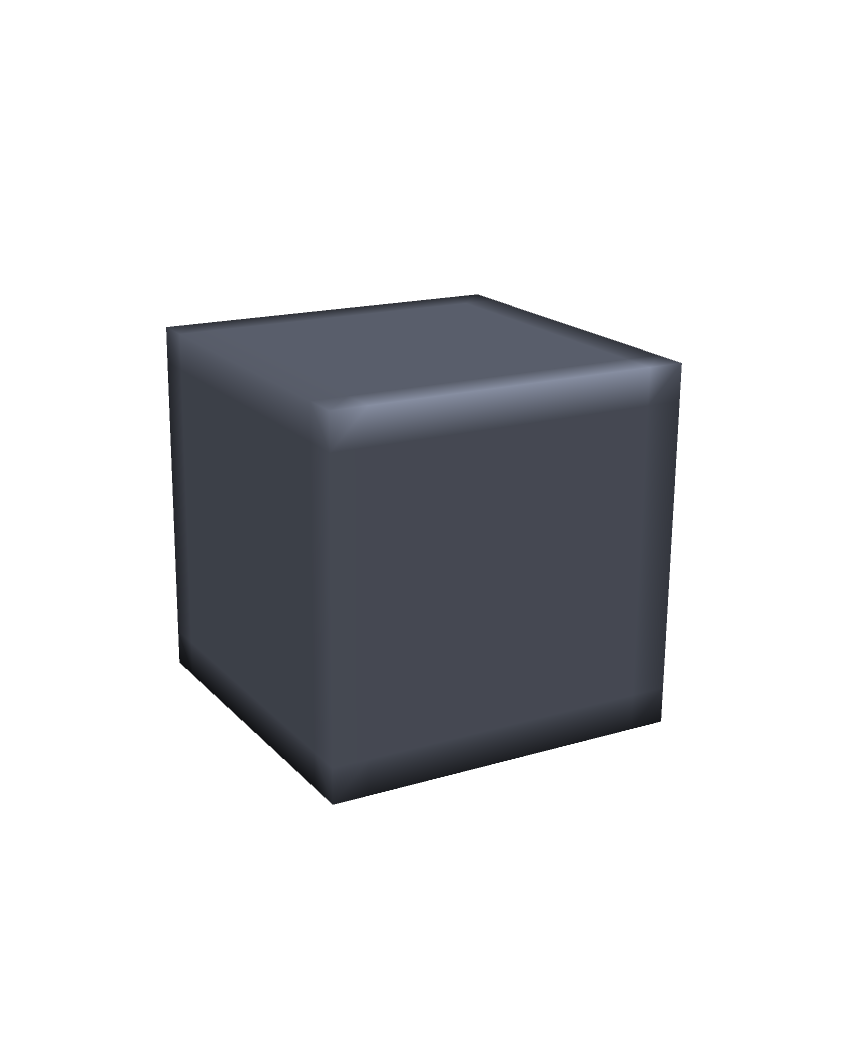
\includegraphics[width=0.24\textwidth]{resources/hexcli_00.png}
        \hfill
        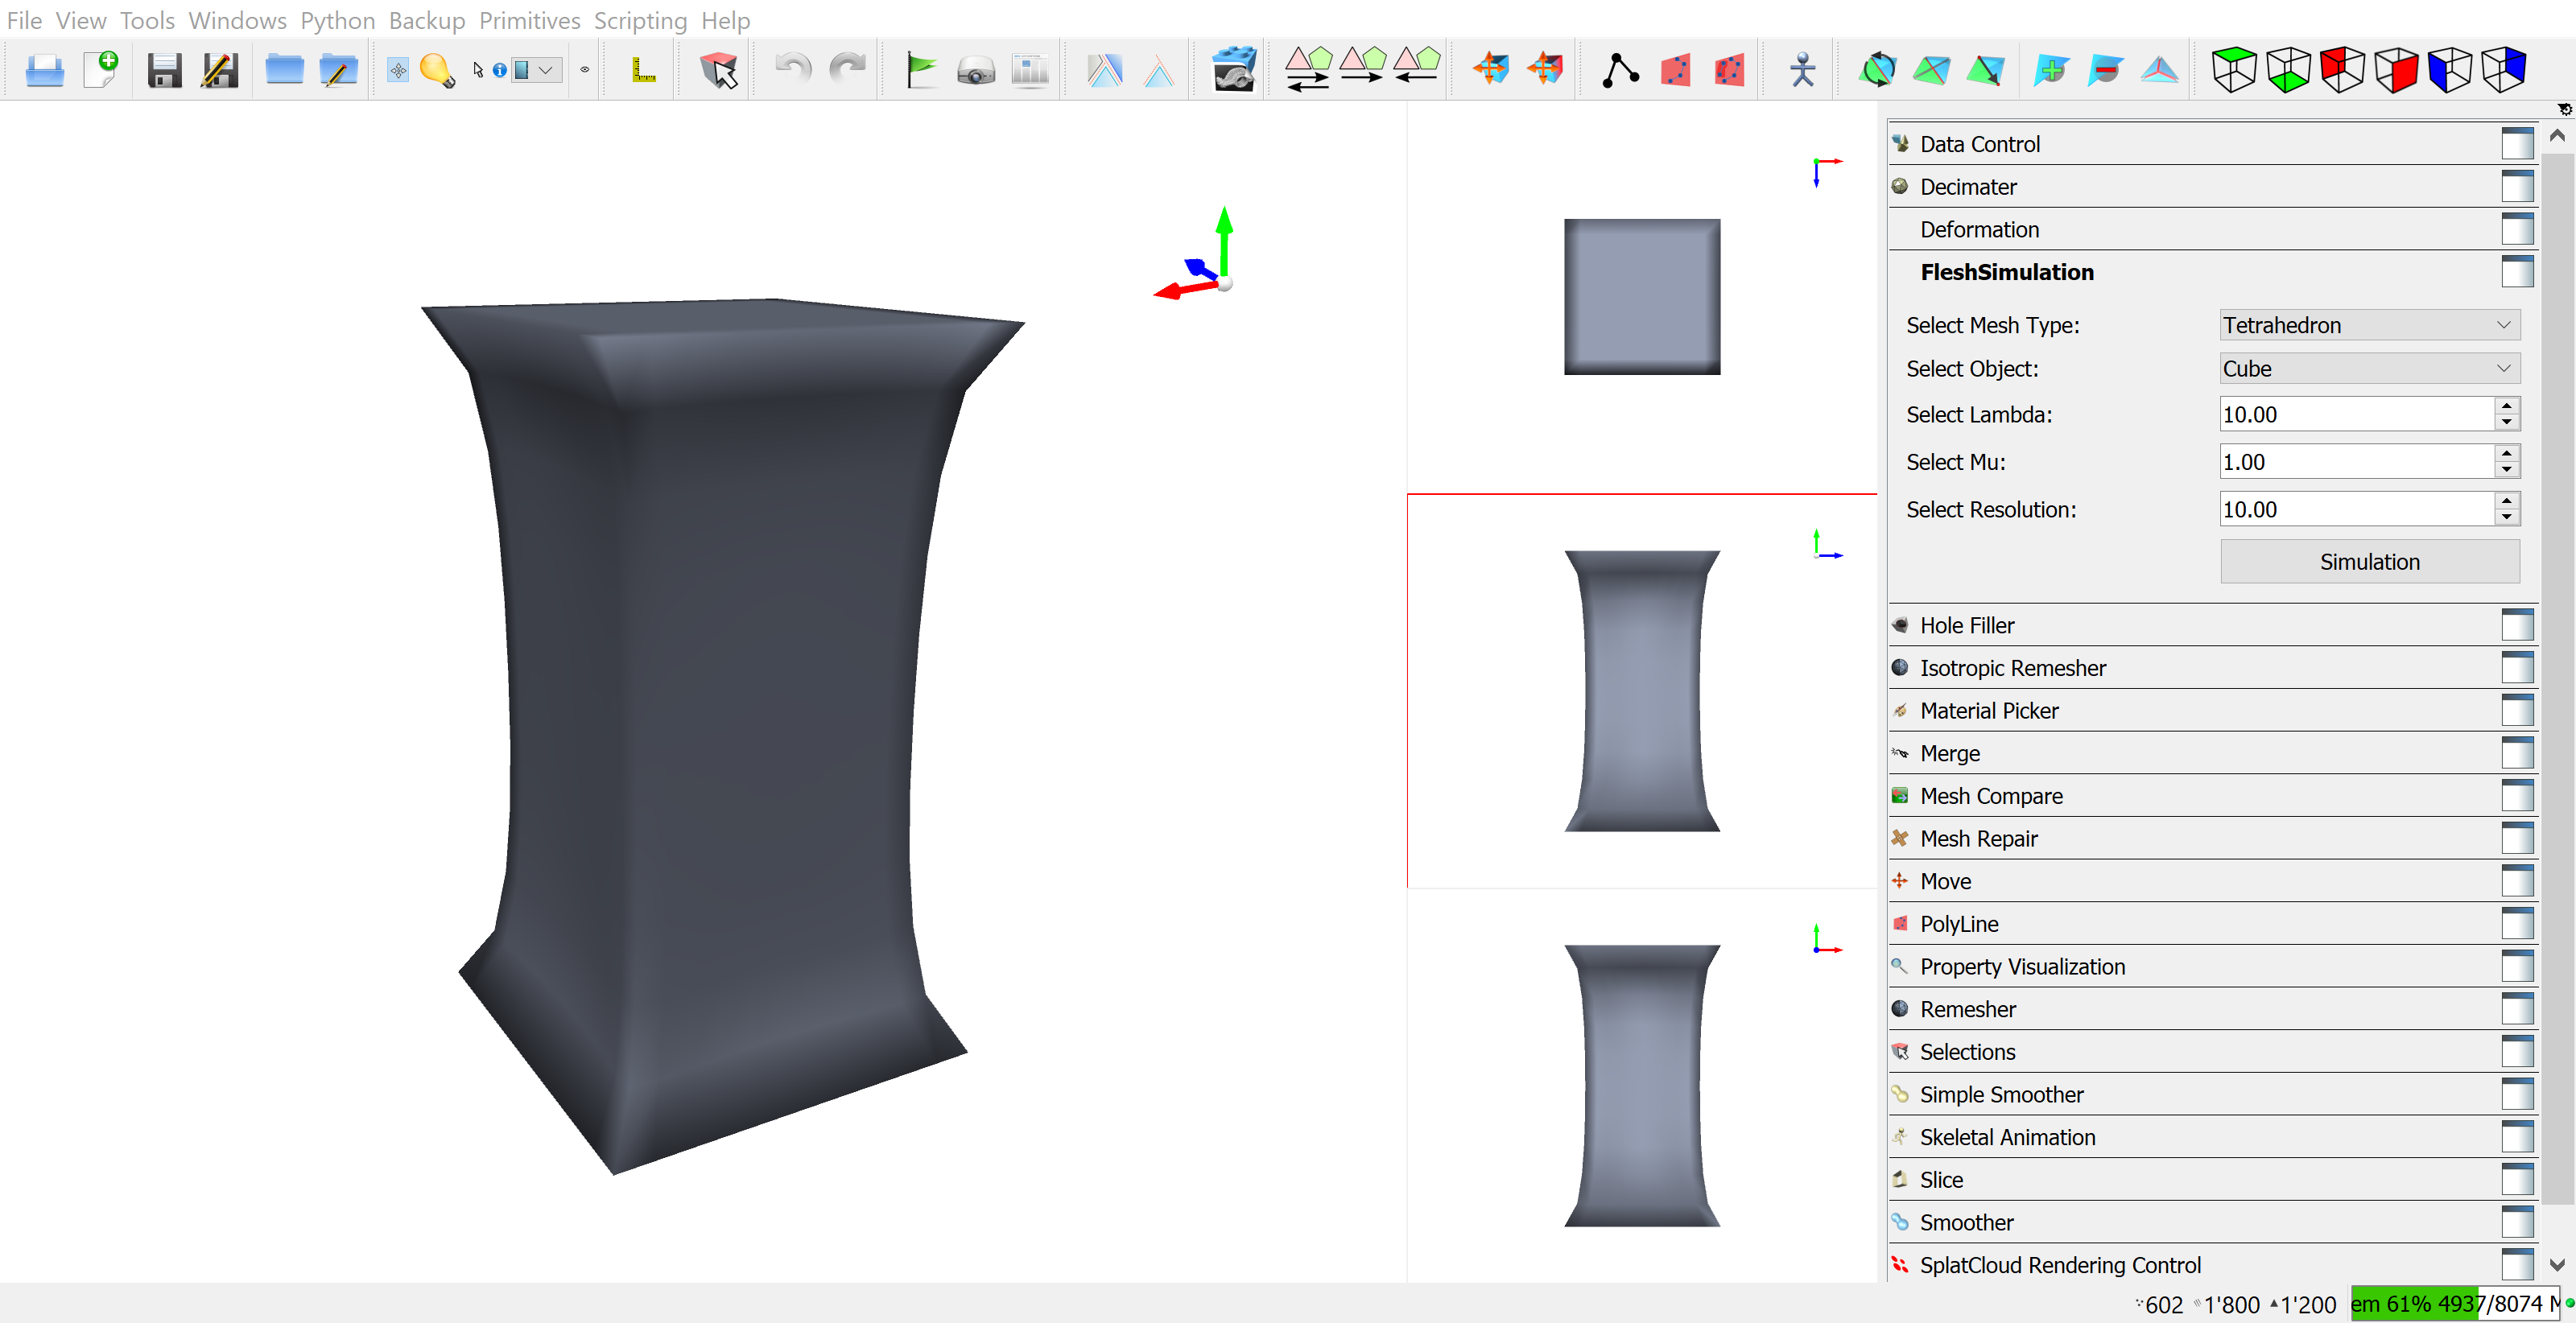
\includegraphics[width=0.24\textwidth]{resources/hexcli_08.png}
        \hfill
        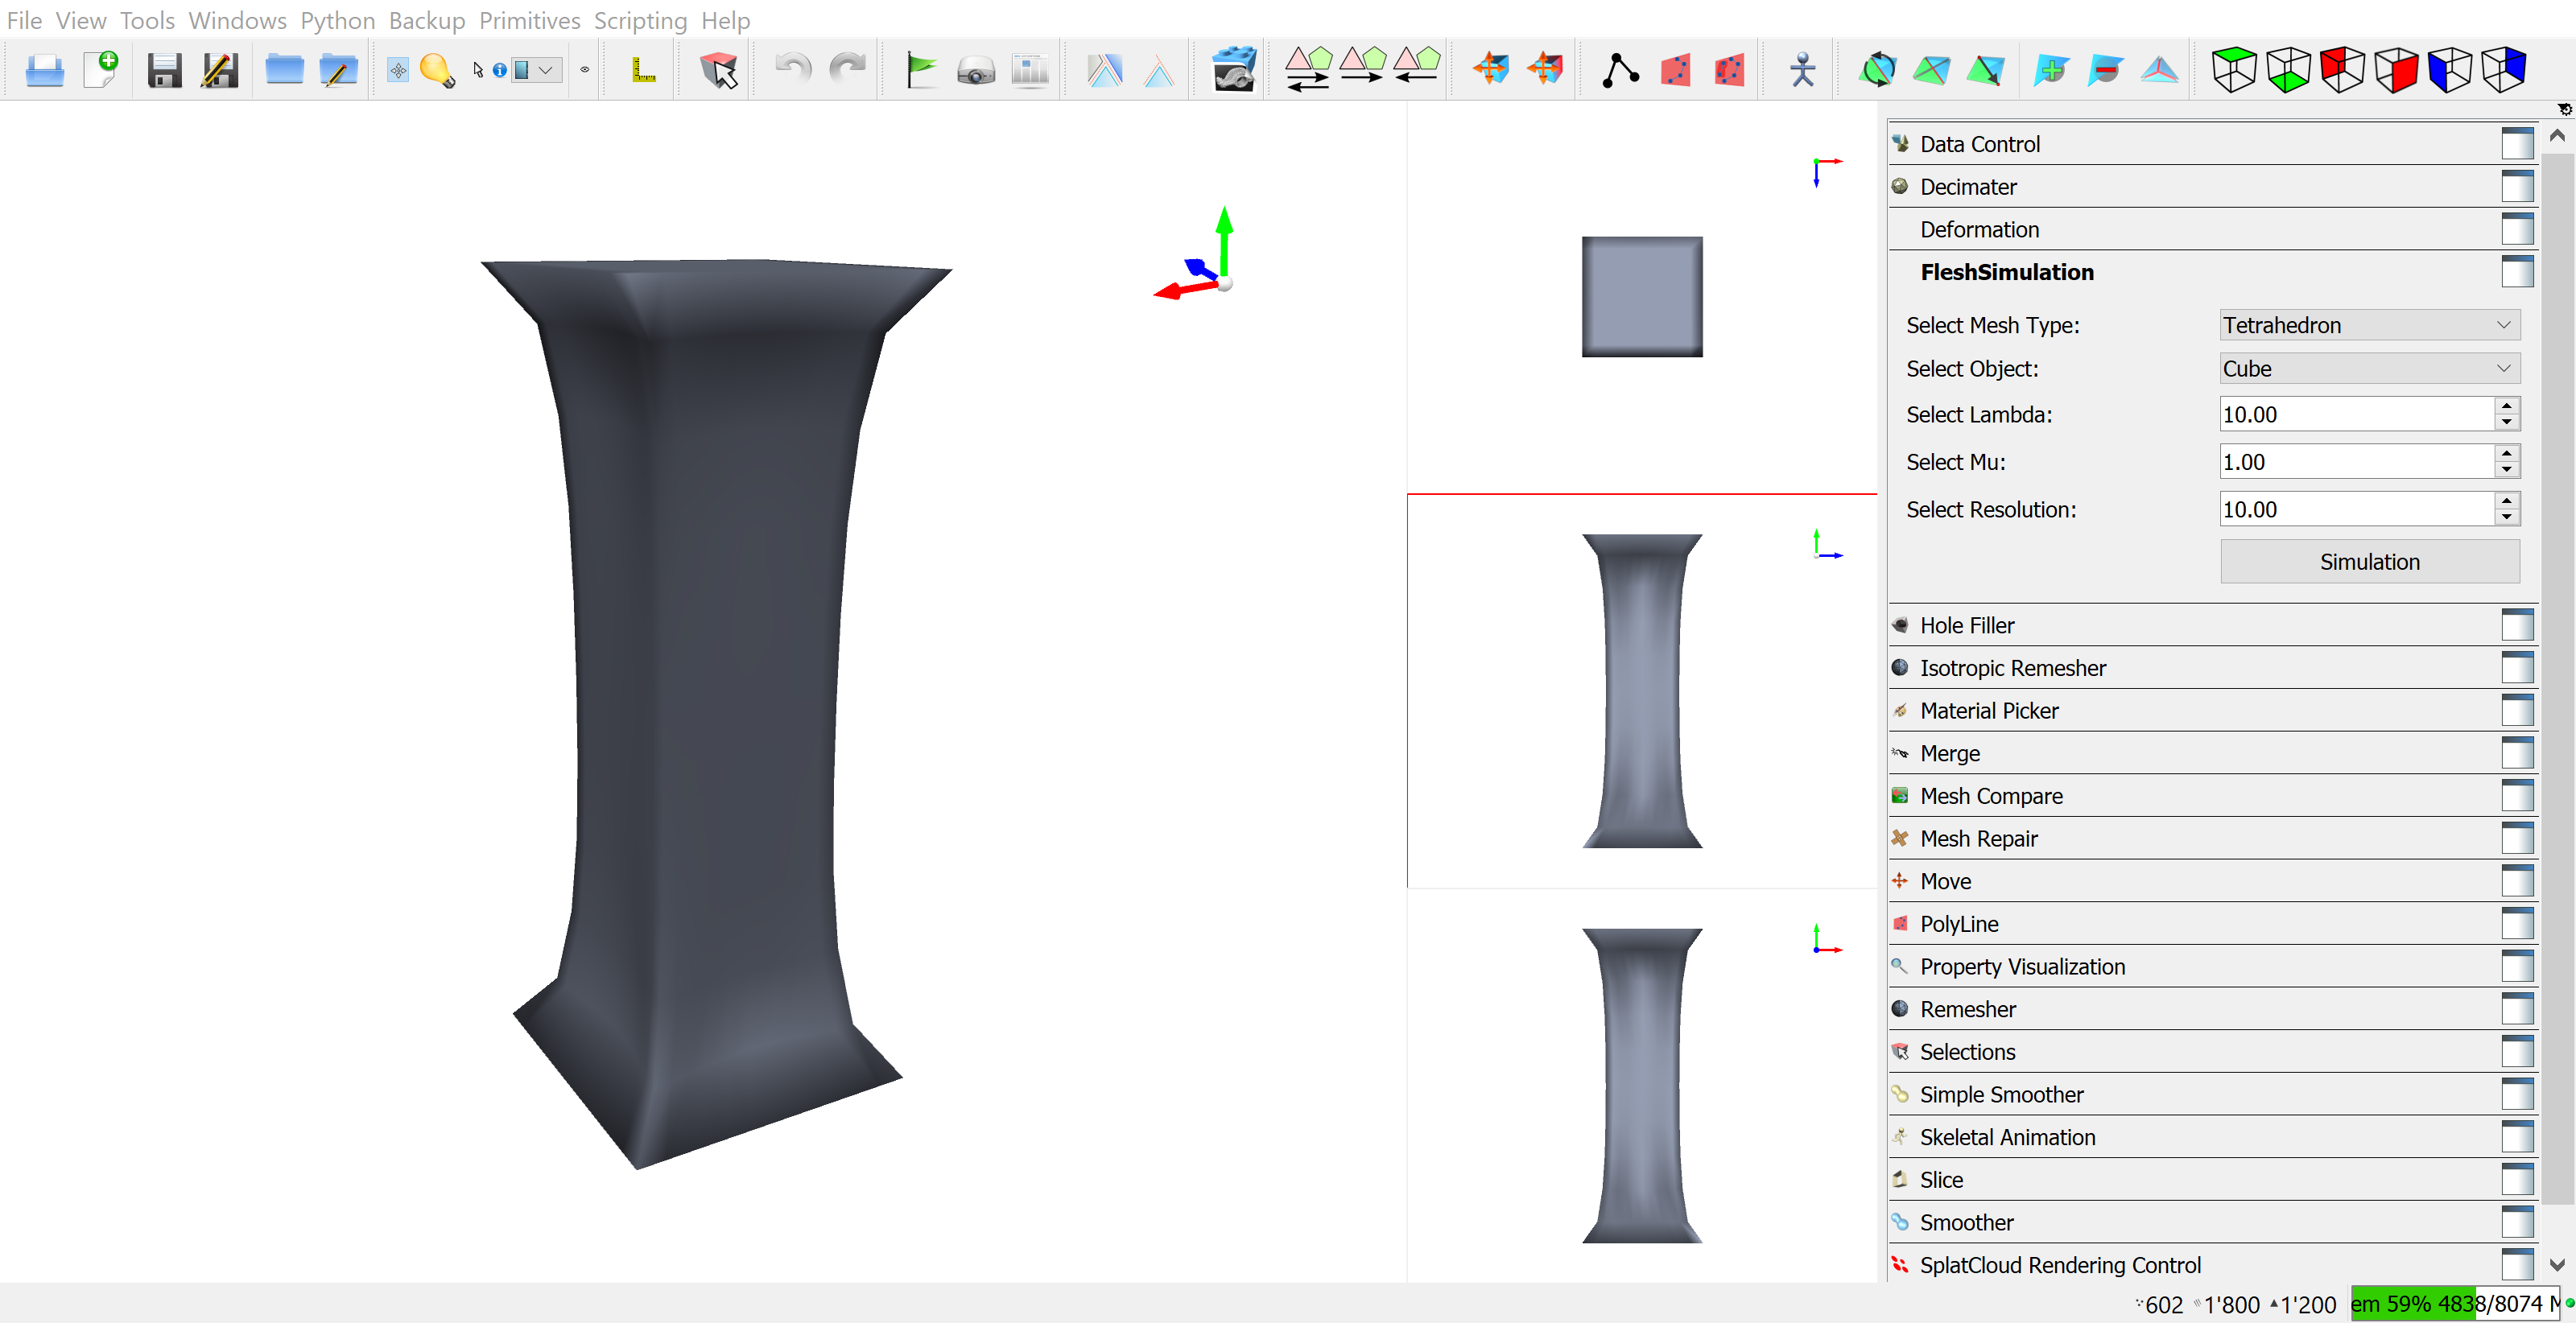
\includegraphics[width=0.24\textwidth]{resources/hexcli_16.png}
        \hfill
        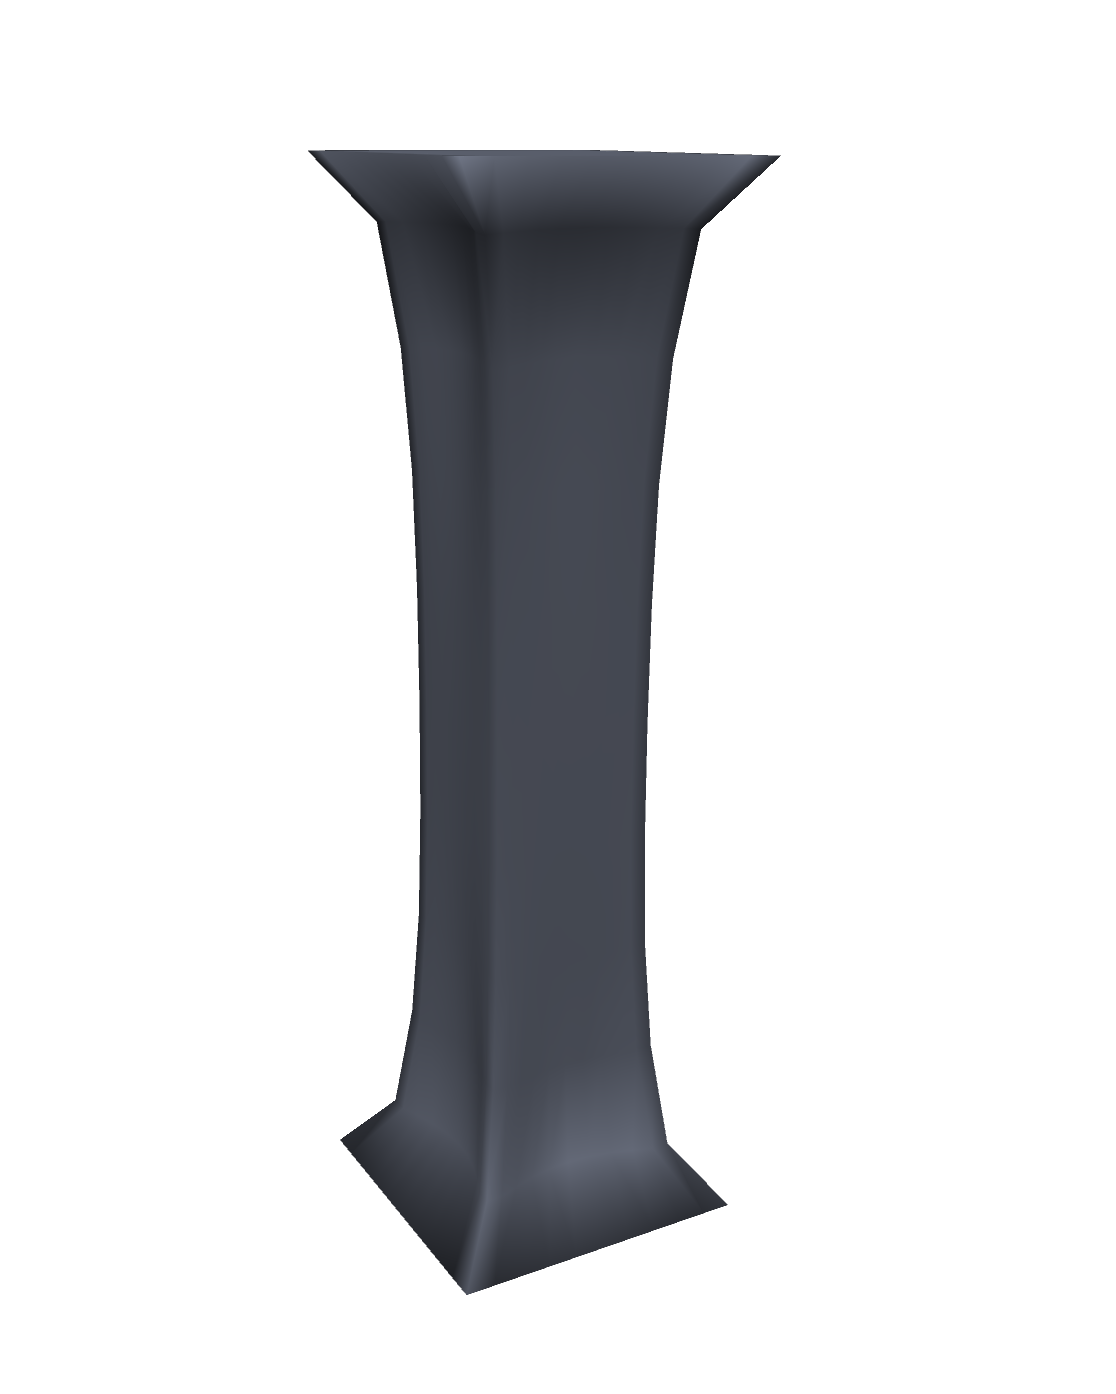
\includegraphics[width=0.24\textwidth]{resources/hexcli_24.png}
        \caption{Stretch test on a hexahedral mesh}
    \end{subfigure}
    \vskip\baselineskip
    \begin{subfigure}[b]{\textwidth}
        \centering
        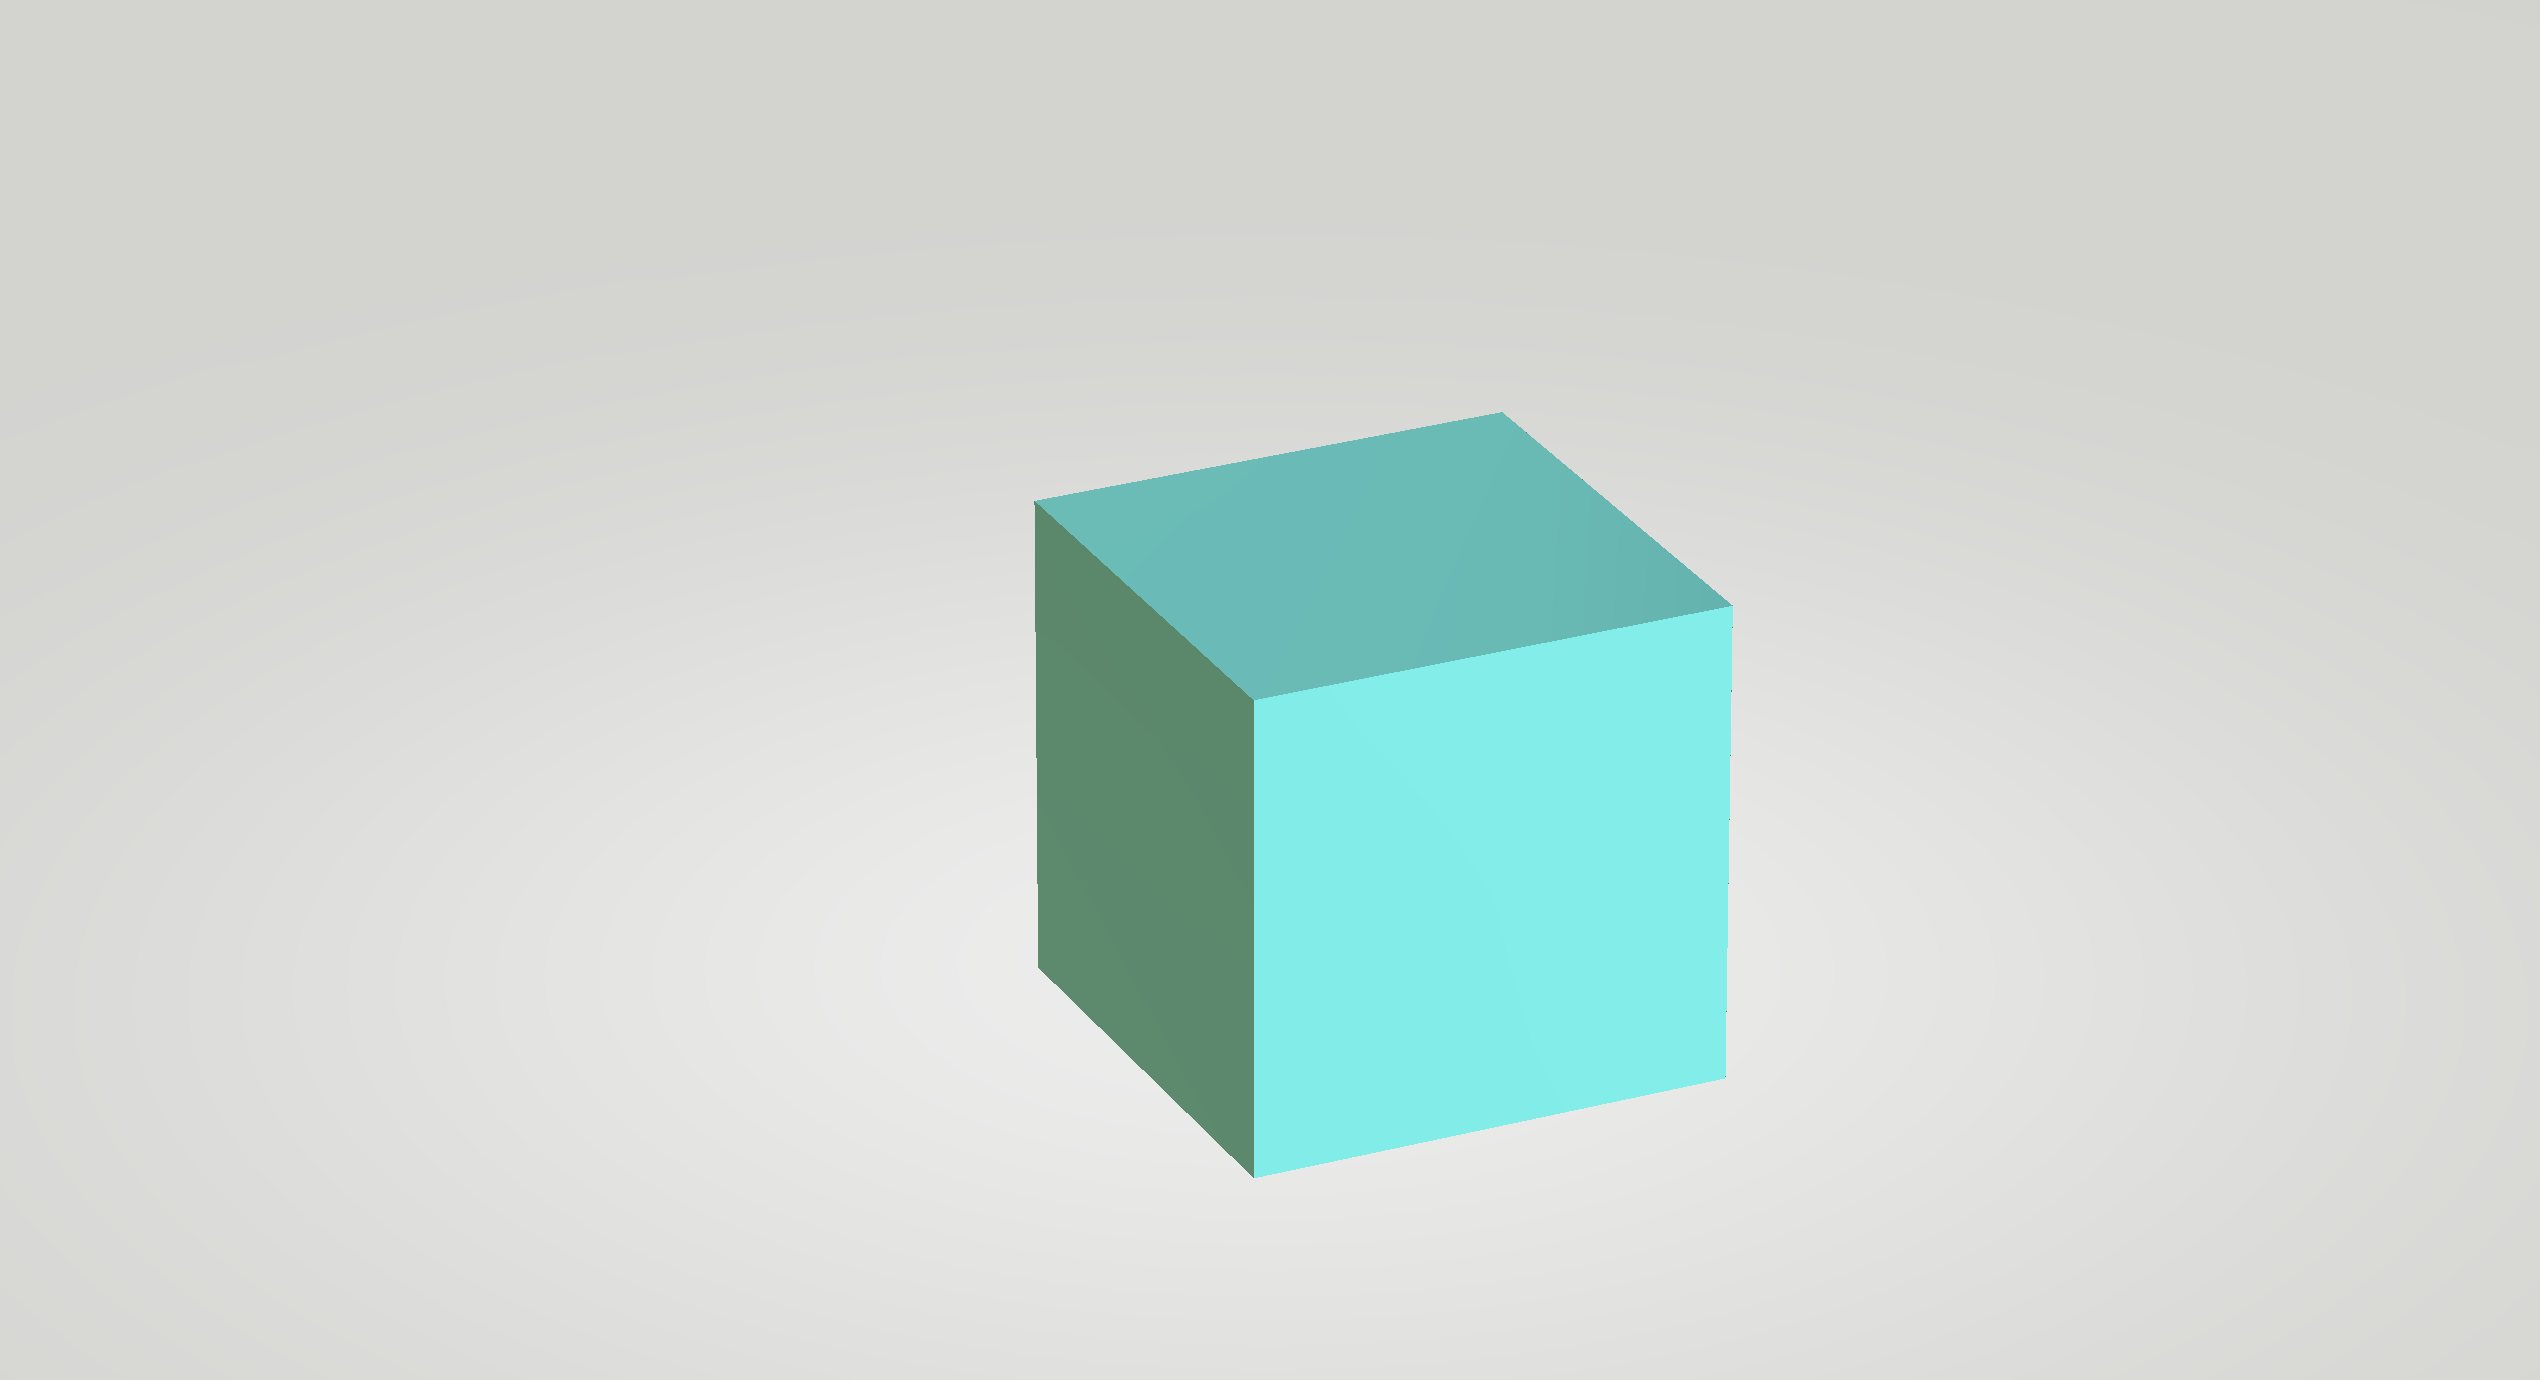
\includegraphics[width=0.24\textwidth]{resources/tetcli_step0.png}
        \hfill
        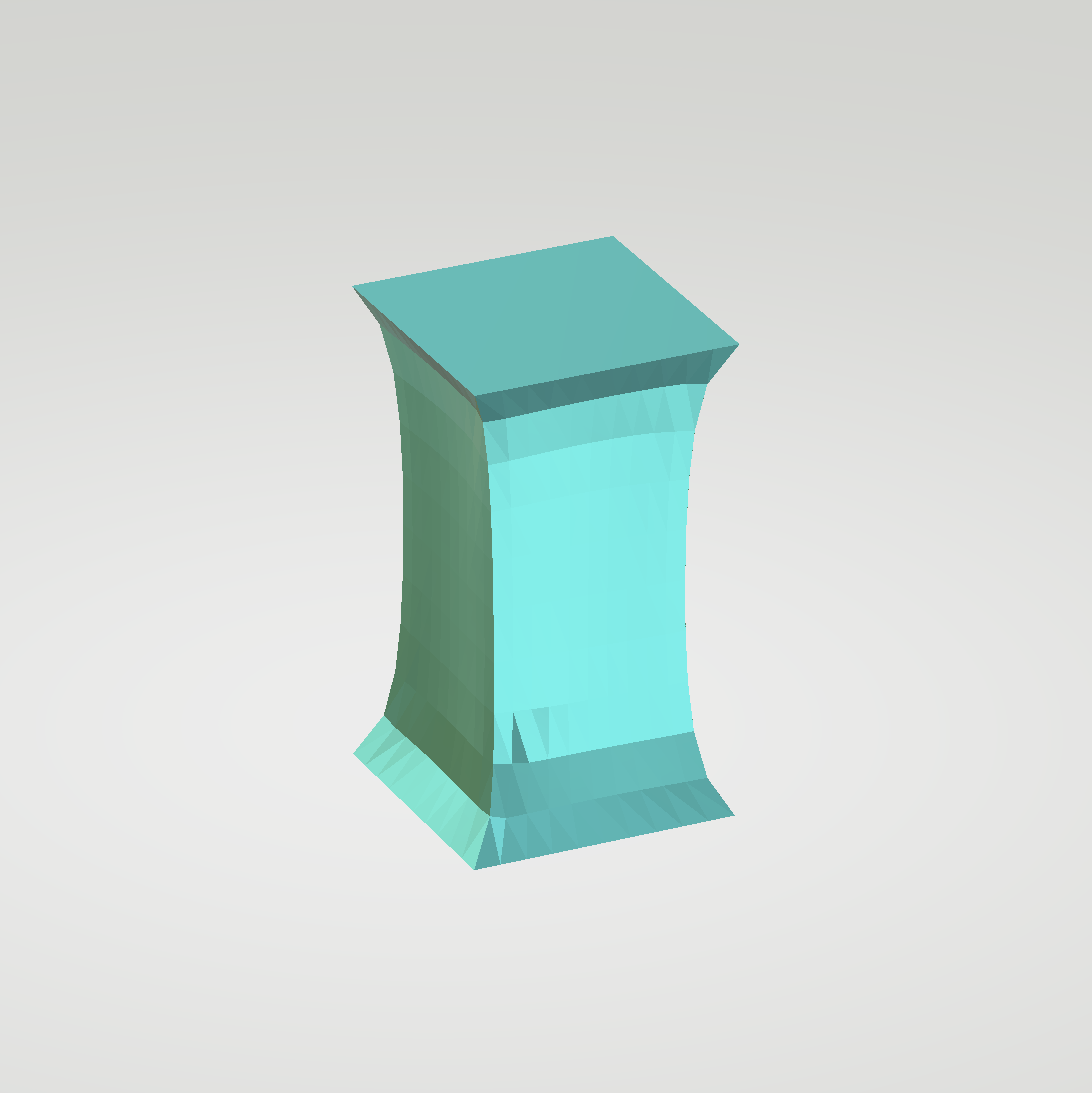
\includegraphics[width=0.24\textwidth]{resources/tetcli_step8.png}
        \hfill
        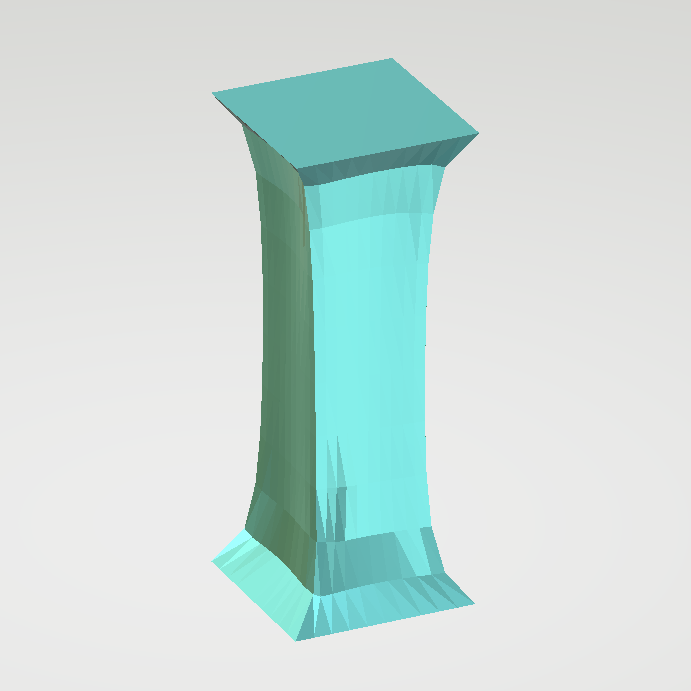
\includegraphics[width=0.24\textwidth]{resources/tetcli_step16.png}
        \hfill
        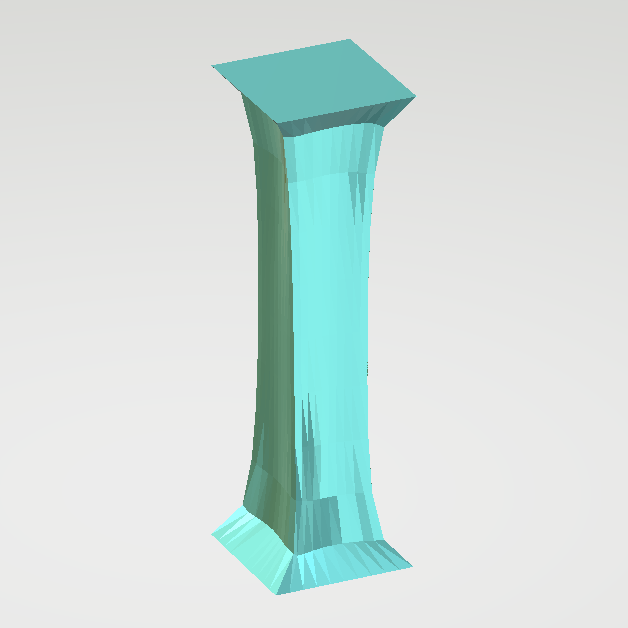
\includegraphics[width=0.24\textwidth]{resources/tetcli_step24.png}
        \caption{Stretch test on a tetrahedral mesh}
    \end{subfigure}
    \caption[Stretch test performed on a cube]{Stretch test performed on a cube with (a) a hexahedral mesh and (b) a tetrahedral mesh}
    \label{fig:stretchtest}
\end{figure}


\todoredefined[inline]{
TODO: Load into OpenFlipper and screenshot results. Include remaining examples (diff. lamé param. and changes in method) and what went right and what went wrong.
}



\section{Discussion}
Stuff, Taylor approx.


